\documentclass[livre]{udes-genie-these}

\usepackage[T1]{fontenc}
\usepackage{booktabs}
\usepackage{url}  % Enables the use of \url{}
\usepackage{graphicx}
\usepackage{color,soul}
\usepackage{lscape} % For landscape orientation

\ConfigurationDocument
{
  langue = francais,
  type = dprmaitrise,
  programme = electrique,
  lignes,
  liste-figures,
  % liste-tableaux,
  fichier-resume-francais = {resume-francais},
  %fichier-resume-anglais = {resume-anglais},
  % fichier-remerciements = {merci},
  % fichier-lexique = {lexique},
  % fichier-symboles = {symboles},
  fichier-acronymes = {acronymes},
  fichiers-references = {references},
  auto-bib,
  style-references = plain,
}

\TitreFrancais{L'IA AU SERVICE DU MONTAGE VIDÉO: UTILISATION DES LLMS POUR SÉLECTIONNER DES MOMENTS FORTS ET OPTIMISER L'ENGAGEMENT}
\Auteur{Alexandre}{LAFLEUR}
\Date{Décembre}{2024}
\MotsClesFrancais{Intelligence artificielle, montage vidéo, LLM}

\Directeur{François}{GRONDIN}
\Evaluateur{François}{MICHAUD}
\Evaluateur{François}{FERLAND}

\begin{document}

\chapter{INTRODUCTION}

L'essor des plateformes sociales comme Instagram et YouTube, et plus récemment les formats courts de YouTube Shorts et Reels sur Instagram, a bouleversé la manière dont le contenu vidéo est consommé. La demande croissante pour des contenus courts, dynamiques et engageants impose de nouvelles exigences aux créateurs, qui doivent non seulement produire du contenu de qualité, mais également répondre à des attentes de rapidité et de répétition pour captiver l'audience. Des plateformes telles que Captions.ai et Ssemble, par exemple, ont été développées pour répondre à ces besoins en facilitant l'extraction et la personnalisation rapides de clips courts, spécifiquement adaptés à des plateformes sociales populaires \cite{captions2024}\cite{ssemble2024}.
La création manuelle de clips courts nécessite une sélection minutieuse des moments saillants, des éléments narratifs forts, et une attention à la fluidité entre les séquences. Cependant, bien que des outils comme 2short.ai permettent l'automatisation de cette sélection en identifiant les moments les plus captivants grâce à des technologies de suivi facial et d'analyse de l'engagement \cite{short2024}, ils sont souvent limités dans leur capacité à capturer des nuances narratives complexes. Ceci demande un investissement en temps conséquent, que de nombreuses équipes de créateurs de contenu, petites entreprises ou même grandes marques, ne peuvent se permettre. Ainsi, l'automatisation du montage vidéo devient une nécessité pour produire efficacement des contenus captivants et pertinents sans sacrifier la qualité \cite{munch2024}.

Pour produire un grand volume de contenu, de nombreux influenceurs choisissent de faire appel à des monteurs privés ou à des agences spécialisées qui prennent en charge le montage et la publication de leurs vidéos. Bien que cette solution soit efficace, elle s'avère très coûteuse, et la majorité des influenceurs ne dispose pas des moyens financiers pour y recourir régulièrement. En effet, Forbes estime que pour chaque 1 000 vues, YouTube rémunère environ 5 \$, et qu'un créateur doit atteindre au moins un million d'abonnés pour générer environ 60 000 \$ par an. Toutefois, en tenant compte des partenariats avec des marques et d'autres formes de rémunération, le revenu moyen d'un YouTuber s'élève à 68 714 \$ par an selon ZipRecruiter \cite{financebuzz2024}. Même en utilisant les données plus optimistes de ZipRecruiter, il est clair que le salaire d'un youtuber ne permet pas confortablement de payer une agence de marketing ou un monteur. Et pour ceux qui en ont les moyens, une réduction de ces coûts leur permettrait quand même de produire davantage de contenu et d'optimiser leur présence sur les plateformes sociales.
Les influenceurs ont donc besoin d'une alternative qui reproduit le travail des monteurs et agences à un coût plus abordable, sans compromis sur la qualité du contenu. Des plateformes comme Klap et Recast Studio, par exemple, proposent des outils de montage vidéo automatisé, réduisant ainsi la dépendance aux services de montage externes tout en maintenant une qualité adaptée aux réseaux sociaux \cite{klap2024}\cite{recast2024}.
Cependant, ces solutions ne sont pas suffisantes car elles se limitent à remplacer le travail d’un monteur, sans couvrir les fonctions d’une agence. Une agence ne se contente pas de monter des vidéos, elle prend également en charge leur création, leur publication, et surtout leur optimisation en fonction des tendances émergentes. Cette capacité d’apprentissage constant permet aux agences de rester à l’avant-garde des nouvelles pratiques et styles qui maximisent l’impact des vidéos.
À la différence de ces outils, la solution proposée exploite des données multimodales et teste systématiquement la performance des vidéos en temps réel. En créant plusieurs versions d’un même contenu, avec des variations de clips et de montages, elle permet d’isoler précisément les facteurs qui influencent les résultats, garantissant un apprentissage et une adaptation continus.
La solution explorée dans cette recherche vise à utiliser des intelligences artificielles de type LLM pour remplacer le travail des monteurs et des agences. L'objectif est de réduire les coûts en minimisant la main-d'œuvre humaine, tout en assurant un niveau de performance et d'engagement similaire afin de préserver, voire d'améliorer, le nombre moyen de vues par vidéo \cite{ssemble2024}\cite{opusclip2024}.


\chapter{ÉTAT DE L'ART}

\section{Cartographie et analyse critique des travaux de recherche existants}
\subsection{Contexte et Objectifs de l'IAd}	
L'objectif de l'IAd est de fournir une solution automatisée de montage vidéo, qui soit capable de sélectionner les segments les plus pertinents d'une vidéo en fonction de critères de qualité narrative et visuelle, tout en alignant les choix sur les préférences et attentes des spectateurs. Une telle IA serait capable de réaliser plusieurs tâches essentielles : identifier et extraire les moments clés, structurer une narration cohérente, répondre aux préférences spécifiques et aux tendances et offrir une solution rapide et évolutive.
L'IAd doit être capable de comprendre et de localiser les segments d'une vidéo qui ont le plus grand potentiel d'engagement, en tenant compte de l'audience cible et des tendances actuelles \cite{bain2022}. Pour ce faire, elle doit intégrer des méthodes avancées de détection de saillance, de correspondance de texte-image, et d'analyse contextuelle \cite{weng2024}\cite{anonymous2023_bubogpt}. 
Pour faire le montage de ces segments, les clips sélectionnés doivent maintenir une continuité narrative, avec une transition fluide entre les moments. Ceci nécessite une compréhension contextuelle des segments choisis et une capacité à les organiser selon un ordre logique et attractif pour le public \cite{feng2023}\cite{munasinghe2023_pgvideo}. 
Pour augmenter le potentiel d'engagement, la personnalisation devient un atout majeur dans le montage vidéo, permettant à l'IAd d'adapter ses choix en fonction des préférences spécifiques des spectateurs ou des demandes des créateurs. Ceci inclut la prise en compte des signaux de tendance sur les plateformes, tels que les thèmes visuels et sonores populaires \cite{anonymous2023_valley}\cite{captions2024}. 
Pour répondre aux exigences des réseaux sociaux, où la rapidité de publication est essentielle, l'IAd doit être capable de traiter rapidement de grandes quantités de contenu vidéo. Elle doit donc intégrer des techniques d'optimisation de données pour assurer une sélection rapide et efficace des segments \cite{wang2024_hawkeye}\cite{wang2024_lave}. 
En résumé, l'IAd a pour mission de réduire le fardeau du montage manuel tout en produisant des montages qui maximisent l'engagement. Ce projet s'appuie sur des techniques avancées de modélisation multimodale et de compréhension vidéo \cite{zhang2023}\cite{tang2023}, que nous explorerons dans les sections suivantes pour constituer une base technologique solide pour le développement de cette IA.

\subsection{Modélisation Vidéo-textuelle et multimodale pour la sélection de clips}
Pour remplir pleinement sa fonction de montage automatique, l'IAd doit être capable d'analyser et de comprendre le contenu vidéo non seulement en termes d'images mais également en intégrant les éléments textuels et auditifs. Cette section explore les modèles et techniques vidéo-textuelles et multimodales qui permettent d'enrichir la pertinence et la précision de la sélection des segments dans le cadre de l'automatisation du montage.
Des modèles comme CLIP et BuboGPT jouent un rôle fondamental dans la correspondance entre le contenu visuel et les descriptions textuelles \cite{bain2022}\cite{anonymous2023_bubogpt}. CLIP (Contrastive Language-Image Pre-training) a été développé pour relier directement des images à des textes, permettant une correspondance directe entre des concepts visuels et des descriptions narratives. Cette capacité est précieuse pour un montage automatique, car elle permet à l'IAd de sélectionner les segments visuels les plus pertinents par rapport aux requêtes textuelles ou aux tendances narratives \cite{chen2023}\cite{ghosh2019_excl}. Cependant, CLIP est principalement entraîné sur des images statiques, ce qui limite sa capacité à traiter efficacement les dimensions temporelles et narratives des vidéos. Dans un montage vidéo, la continuité visuelle et le contexte narratif sont essentiels, et cette lacune peut réduire la pertinence des segments identifiés.
BuboGPT, quant à lui, renforce cette capacité en ajoutant une couche d'ancrage visuel, permettant une identification et une localisation précises des objets dans chaque image en fonction des descriptions textuelles \cite{feng2023}\cite{munasinghe2023_pgvideo}. Par exemple, une scène de nature pourrait être identifiée et extraite si elle est associée à un texte comme « aventure en plein air ». Cette granularité fine est un atout, mais elle dépend fortement de la qualité des descriptions textuelles fournies. Si les textes sont vagues, ambigus ou contradictoires, le modèle risque de sélectionner des segments non pertinents, réduisant ainsi l'efficacité du montage.
En associant CLIP et BuboGPT, l'IAd pourrait exploiter la force de l'ancrage visuel pour sélectionner des séquences vidéo qui sont en parfaite adéquation avec les attentes narratives, même si elles sont visuellement complexes. CLIP apporte une compréhension générale du lien image-texte, tandis que BuboGPT affine cette compréhension en se concentrant sur des éléments visuels spécifiques \cite{chen2023}\cite{you2023_ferret}. Cependant, l'interopérabilité de ces deux modèles peut poser des défis, notamment en termes de gestion des conflits éventuels entre leurs recommandations respectives.
Si l'image et le texte offrent des informations importantes pour la sélection des segments, l'intégration de l'audio permet une compréhension encore plus riche de la vidéo \cite{anonymous2023_videollama}\cite{han2024_clip}. Les modèles Valley et Video-LLaMA démontrent comment des signaux auditifs peuvent être exploités en parallèle des indices visuels et textuels pour un alignement complet des modalités \cite{huang2024_vtimellm}\cite{anonymous2023_valley}. Valley utilise un alignement multimodal qui intègre des signaux audio pour fournir une compréhension contextuelle approfondie des vidéos, tandis que Video-LLaMA emploie des modules spécialisés qui séparent et intègrent les indices visuels et auditifs en requêtes interprétables par les modèles de langage \cite{xu2024}\cite{anonymous2023_valley}. Cette approche permet de prendre en compte des éléments sonores tels que les dialogues, les changements d'intonation et la musique, qui influencent fortement l'engagement émotionnel et narratif.
Cependant, l'efficacité de ces modèles dépend de la qualité des signaux audio disponibles. Par exemple, dans des environnements bruités ou des vidéos amateurs, la performance de Valley peut diminuer, compromettant ainsi la précision de l'analyse contextuelle. De plus, Video-LLaMA, bien que très performant, est coûteux en termes de calcul, ce qui peut le rendre moins adapté à des vidéos longues ou à des systèmes nécessitant des réponses en temps réel. Une version plus légère et optimisée pourrait être envisagée pour répondre aux contraintes de production.
La fusion multimodale de ces approches (image-texte-audio) ouvre la voie à une sélection de clips qui ne se limite pas aux caractéristiques visuelles d'une vidéo, mais qui intègre une compréhension complète des signaux auditifs et textuels \cite{wang2024_hawkeye}\cite{anonymous2017_localizing}. Cette capacité multimodale est cruciale pour l'IAd, car elle permet de capter l'essence de la narration dans chaque segment et de s'assurer que les extraits choisis correspondent parfaitement aux attentes des spectateurs et aux objectifs narratifs de la vidéo. Néanmoins, l'intégration de multiples modalités peut également introduire des biais ou des conflits entre les signaux. Par exemple, une musique dramatique superposée à des visuels calmes pourrait créer une ambiguïté dans l'interprétation de la scène. La capacité des modèles à hiérarchiser ces signaux ou à arbitrer entre eux reste un défi à relever.
L'utilisation combinée des techniques de CLIP, BuboGPT, Valley, et Video-LLaMA assure que l'IAd bénéficie d'une modélisation vidéo-textuelle sophistiquée capable d'interpréter, de détecter et de structurer les segments les plus engageants en fonction des modalités multiples présentes dans une vidéo \cite{chen2023}\cite{anonymous2023_videollama}\cite{xu2024}\cite{wang2024_hawkeye}. Cependant, pour garantir une performance optimale, ces modèles devront être ajustés sur des données représentatives des besoins spécifiques du projet, en prenant en compte les défis d'interopérabilité, de robustesse aux signaux bruités, et de cohérence narrative.

\subsection{Localisation et segmentation temporelle des moments clés}
Pour garantir une continuité narrative et un montage fluide, l'IAd doit être capable d'identifier non seulement les moments clés dans une vidéo, mais également leurs limites temporelles précises. Les techniques de localisation temporelle et de segmentation des vidéos jouent ici un rôle essentiel, permettant à l'IA de découper les séquences tout en conservant leur sens et en respectant la chronologie narrative. Cette section explore les approches avancées de segmentation temporelle et de localisation des moments clés, nécessaires pour une sélection précise et cohérente.
Les modèles comme VTimeLLM et VTG-LLM (\textit{Video Temporal Grounding}) apportent des solutions novatrices pour la délimitation précise des segments vidéo en intégrant des indicateurs temporels explicites \cite{huang2024_vtimellm}\cite{guo2024_vtgllm}. VTimeLLM, par exemple, utilise une stratégie d'entraînement en plusieurs étapes pour renforcer la précision temporelle, permettant de mieux comprendre les débuts et fins des segments d'intérêt \cite{han2024_clip}\cite{lei2021_clipbert}.
VTG-LLM, quant à lui, exploite des embeddings de séquence-temps et des jetons de temps absolus pour ancrer précisément les moments dans le temps, évitant ainsi les erreurs de quantification qui peuvent survenir dans des vidéos complexes ou de longue durée. Cette intégration de l'horodatage permet au modèle de maintenir une continuité temporelle, essentielle pour les montages vidéo nécessitant une précision d'alignement entre les scènes \cite{guo2024_vtgllm}\cite{you2023_ferret}.
Ces modèles démontrent l'importance de la localisation temporelle dans les vidéos longues. En intégrant l'horodatage de manière explicite, l'IAd pourrait non seulement sélectionner les moments clés avec une plus grande précision, mais aussi s'assurer que chaque segment est correctement positionné dans l'ordre narratif, évitant ainsi les coupures abruptes ou incohérentes \cite{lei2021_clipbert}\cite{anonymous2017_localizing}.
Pour organiser les segments dans un ordre fluide, des modèles comme le Moment Context Network (MCN) et 2D-TAN (\textit{Temporal Adjacent Networks})  utilisent des techniques de cartographie temporelle et contextuelle \cite{ghosh2019_excl}\cite{zhang2016_lstm}. MCN associe des caractéristiques locales et globales pour identifier des débuts et fins de moments spécifiques, en analysant non seulement chaque segment individuellement, mais aussi en tenant compte du contexte général de la vidéo \cite{zhang2016_lstm}\cite{zhang2019_memory}.
2D-TAN adopte une approche de cartographie bidimensionnelle pour modéliser les relations temporelles entre segments adjacents, garantissant ainsi que chaque segment sélectionné conserve une continuité narrative par rapport aux autres. Ce modèle est particulièrement efficace dans les vidéos avec une progression d'actions, où chaque moment dépend logiquement de celui qui le précède ou de celui qui le suit \cite{prabhu2017_retrieval}\cite{zhang2020_temporal}.
L'IAd pourrait tirer parti de ces techniques pour maintenir une fluidité dans le montage final en sélectionnant des segments qui s'enchaînent naturellement, renforçant ainsi la cohérence de la narration. Par exemple, dans une vidéo de voyage, l'IA pourrait s'assurer que la transition entre une scène d'introduction d'un lieu et une scène d'exploration de ce même lieu se fasse sans rupture \cite{zhang2016_lstm}\cite{zhang2019_memory}.
L'intégration des techniques de localisation temporelle de modèles comme VTimeLLM, VTG-LLM, MCN, et 2D-TAN permet d'assurer une continuité narrative tout en respectant les limites temporelles des segments d'intérêt \cite{han2024_clip}\cite{lei2021_clipbert}\cite{zhang2016_lstm}\cite{prabhu2017_retrieval}. En appliquant ces approches, l'IAd peut non seulement sélectionner les moments clés, mais également les structurer dans un ordre logique qui maximise l'impact narratif.
Grâce à ces techniques, l'IAd devient capable de découper les séquences de manière précise, d'assembler les moments dans une séquence fluide, et de produire un montage qui maintient l'attention du spectateur tout en assurant la clarté narrative \cite{ghosh2019_excl}\cite{zhang2019_memory}.

\subsection{Détection des faits saillants et filtrage du bruit}
L'IAd doit être capable de repérer les moments saillants et de filtrer les segments de moindre intérêt ou redondants pour éviter de surcharger la vidéo finale et maximiser l'engagement du spectateur. Les modèles explorés dans cette section se concentrent sur la détection des faits saillants et l'élimination des segments non pertinents, permettant ainsi une sélection précise des passages qui ont le plus fort potentiel narratif et visuel.
HL-CLIP et GPTSee sont deux modèles innovants pour la détection des faits saillants. HL-CLIP utilise une technique de regroupement de saillance (\textit{saliency pooling}) pour stabiliser la détection de moments intéressants en moyenne les scores de saillance à travers plusieurs frames adjacents \cite{han2024_clip}\cite{sun2023_gptsee}. Cette approche permet une détection plus robuste des segments pertinents, même dans des séquences complexes, et évite les sélections incohérentes \cite{you2023_ferret}\cite{sun2023_gptsee}.
GPTSee, quant à lui, repose sur une analyse de similarité sémantique entre les descriptions des images extraites et les requêtes textuelles pour identifier les moments saillants les plus engageants \cite{sun2023_gptsee}\cite{liu2022_umt}. En ajoutant un filtrage sémantique, GPTSee affine la sélection pour ne retenir que les segments en lien direct avec les thèmes ou intentions de la narration.
HL-CLIP et GPTSee démontrent comment la détection de faits saillants peut être renforcée par des scores de similarité et de saillance, améliorant ainsi la pertinence des extraits retenus pour le montage. En appliquant une combinaison de ces techniques, l'IAd peut sélectionner les moments les plus impactants tout en minimisant les distractions \cite{han2024_clip}\cite{sun2023_gptsee}.

Dans le domaine du filtrage de contenu, LLoVi (\textit{Language-based Long-range Video question- answering framework}) propose une méthode de résumé multi-étapes pour éliminer le bruit et affiner la qualité des segments choisis. L'approche de LLoVi consiste à générer des descriptions textuelles pour chaque clip court, puis à les résumer en plusieurs étapes pour éliminer les informations redondantes ou non pertinentes \cite{anonymous2023_valley}\cite{zhang2019_memory}. Ce processus de résumé successif permet de concentrer l'attention sur les passages ayant la plus forte valeur narrative.
Pour l'IAd, cette méthode de filtrage multi-étapes pourrait être utilisée pour garantir que chaque segment sélectionné a une valeur ajoutée pour la narration globale, en écartant les éléments non essentiels \cite{zhang2019_memory}\cite{han2024_clip}. Par exemple, dans une vidéo de conférence, l'IA pourrait sélectionner uniquement les moments où des idées clés sont évoquées, en omettant les segments répétitifs ou moins significatifs.
La détection des faits saillants et le filtrage de bruit sont essentiels pour permettre à l'IAd de produire des montages clairs et captivants, où chaque segment choisi sert un but narratif. Les approches de HL-CLIP, GPTSee, et LLoVi offrent des solutions pour optimiser la pertinence et l'impact des sélections \cite{sun2023_gptsee}\cite{han2024_clip}\cite{zhang2019_memory}.
En intégrant ces techniques, l'IAd peut garantir un montage qui retient les moments les plus engageants tout en supprimant les segments redondants ou superflus. Cette capacité à détecter et à filtrer les faits saillants contribue non seulement à maximiser l'impact visuel, mais également à maintenir l'intérêt du spectateur tout au long de la vidéo \cite{sun2023_gptsee}\cite{anonymous2023_valley}.

\subsection{Fusion multimodale et alignement pour une narration cohérente}
Pour qu'un montage vidéo soit percutant et narrativement fluide, l'IAd doit intégrer des informations provenant de plusieurs modalités – visuelle, textuelle, et auditive – en une seule structure cohérente. La fusion multimodale et l'alignement des informations sont donc essentiels pour sélectionner des clips qui se complètent et qui maintiennent un flux narratif logique et engageant. Dans cette section, nous explorons les techniques qui permettent d'enrichir la narration vidéo en utilisant des approches multimodales sophistiquées.
Les modèles UMT et Slot-VLM offrent des solutions complètes pour intégrer des informations visuelles, textuelles, et auditives dans une seule structure cohérente \cite{liu2022_umt}\cite{xu2024}. UMT (Unified Multi-modal Transformers) exploite les données audio et visuelles pour extraire des moments spécifiques en fonction des requêtes textuelles, en intégrant un générateur et un décodeur de requêtes pour transformer les attentes narratives en points de détection temporels \cite{liu2022_umt}. Cette méthode de fusion permet de traiter les vidéos comme un ensemble multimodal complet, assurant que les segments sélectionnés tiennent compte de tous les signaux disponibles.
Slot-VLM introduit une autre dimension avec son système de SlowFast Slots, qui décompose les vidéos en "Slow-Slots" (jetons centrés sur les objets) et "Fast-Slots" (jetons centrés sur les événements) \cite{xu2024}. Cette technique permet d'adapter l'analyse des vidéos selon la fréquence d'apparition des objets et la dynamique temporelle des événements, en maintenant une cohérence entre les objets fixes et les mouvements rapides. Cette approche est particulièrement utile pour une narration fluide, car elle prend en compte les éléments stables (comme les décors) et les éléments en mouvement, assurant une transition naturelle entre les segments.
En appliquant des techniques similaires de fusion multimodale, l'IAd peut analyser des segments audio-visuels en fonction des indices narratifs et de l'engagement attendu. Par exemple, dans une vidéo d'événements, le son d'un applaudissement et le mouvement des foules peuvent être utilisés conjointement pour déterminer un point saillant, créant ainsi un moment de forte intensité émotionnelle \cite{xu2024}\cite{liu2022_umt}.
Les modèles ExCL (\textit{Extractive Clip Localization}) et QD-DETR (\textit{Query-Dependent DEtection TRansformer}) permettent d'adapter dynamiquement les choix de segments en fonction des descriptions narratives et des requêtes textuelles \cite{ghosh2019_excl}\cite{sun2023_gptsee}. ExCL utilise une approche extractive qui prédit les frames de début et de fin en fonction de la pertinence avec les descriptions narratives. Ceci permet de sélectionner des segments qui s'alignent étroitement avec les attentes narratives, assurant que chaque clip choisi apporte une valeur ajoutée à la continuité de l'histoire \cite{ghosh2019_excl}.
QD-DETR utilise un encodeur à attention croisée qui intègre explicitement les requêtes dans la représentation des clips vidéo, offrant un niveau d'adaptabilité élevé pour correspondre précisément aux intentions narratives des spectateurs \cite{lei2021_moments}. Grâce à un mécanisme de matching flexible, il est possible de discriminer entre les segments en fonction de la demande, filtrant les moments qui ne correspondent pas aux critères recherchés.
Avec des techniques d'alignement et d'adaptabilité, l'IAd peut adapter ses choix de segments en temps réel en fonction des tendances actuelles ou des préférences de l'utilisateur \cite{ghosh2019_excl}\cite{lei2021_moments}. Par exemple, si un clip est sélectionné pour répondre à une tendance spécifique sur les réseaux sociaux, l'IA pourra ajuster les critères de sélection pour maximiser l'engagement du spectateur, en s'assurant que le contenu est toujours aligné avec les attentes narratives.
La combinaison des approches de fusion multimodale et d'alignement permet à l'IAd de construire une narration visuellement et contextuellement riche, en sélectionnant des clips qui se complètent sur le plan visuel, textuel et auditif. Les modèles UMT, Slot-VLM, ExCL, et QD-DETR démontrent que l'intégration des modalités permet d'assurer que chaque segment choisi respecte non seulement le contenu, mais également le contexte et l'intention narrative \cite{liu2022_umt}\cite{xu2024}\cite{ghosh2019_excl}\cite{lei2021_moments}.
En utilisant des techniques de fusion et d'alignement, l'IAd peut structurer un montage vidéo qui attire l'attention tout en offrant une continuité narrative. Cette intégration multimodale est cruciale pour garantir une cohérence dans le montage final, maximisant l'impact des segments retenus et permettant de maintenir un intérêt constant pour le spectateur \cite{liu2022_umt}\cite{xu2024}\cite{ghosh2019_excl}.

\subsection{Optimisation des modèles et traitement des vidéos longues}
Dans le montage vidéo, en particulier pour les vidéos de longue durée, il est essentiel d'optimiser les ressources sans compromettre la précision de la sélection des segments. L'IAd doit non seulement pouvoir identifier les moments clés dans des vidéos longues, mais elle doit aussi le faire de manière efficace et rapide. Les modèles explorés dans cette section se concentrent sur des techniques d'optimisation qui permettent un traitement plus rapide et moins gourmand en ressources, tout en maintenant une sélection de clips pertinente.
Les modèles LongVLM et Less is More (CLIPBERT) mettent en avant des techniques d'échantillonnage éparse et de segmentation optimisée pour éviter le traitement de chaque frame dans les vidéos longues \cite{weng2024}\cite{lei2021_clipbert}. LongVLM segmente les vidéos longues en clips courts et extrait pour chaque segment les caractéristiques locales, avant de les fusionner dans un contexte global \cite{weng2024}. Cette approche réduit le volume de données à traiter tout en maintenant une compréhension précise des segments.
CLIPBERT, quant à lui, utilise un échantillonnage éparse pendant l'entraînement pour capturer les informations essentielles tout en réduisant les besoins en mémoire. Lors de l'inférence, CLIPBERT applique un échantillonnage dense, permettant ainsi de conserver un haut niveau de précision dans la sélection des moments saillants sans traiter chaque frame individuellement \cite{lei2021_clipbert}.
En utilisant des méthodes d'échantillonnage et de segmentation, l'IAd peut traiter les vidéos longues de manière efficace, en s'assurant que seuls les segments pertinents sont extraits. Par exemple, dans un documentaire ou un long film, cette optimisation permet de cibler des moments clés sans engorger les ressources de traitement \cite{weng2024}\cite{lei2021_clipbert}.
Les modèles VTG-LLM et VTimeLLM utilisent des techniques de compression des données visuelles pour réduire la surcharge de traitement sans sacrifier la qualité de l'information \cite{guo2024_vtgllm}\cite{huang2024_vtimellm}. VTG-LLM introduit une compression par slot qui regroupe les informations visuelles en blocs, permettant un échantillonnage étendu avec une capacité de traitement plus élevée \cite{guo2024_vtgllm}. Cette technique est particulièrement utile pour les vidéos longues et complexes, où chaque bloc compressé conserve des détails essentiels pour la narration.
VTimeLLM, de son côté, utilise une stratégie d'entraînement par étapes pour améliorer la localisation temporelle dans des vidéos longues, permettant ainsi de mieux appréhender les séquences d'événements sans pertes de données importantes \cite{huang2024_vtimellm}. Grâce à des jetons compressés, ce modèle permet de traiter des vidéos volumineuses tout en conservant une précision optimale.
En utilisant des techniques de compression et de traitement par slots, l'IAd peut gérer de grandes quantités de données sans ralentir le processus de sélection, tout en assurant la précision nécessaire pour maintenir l'intérêt narratif et visuel des clips \cite{guo2024_vtgllm}\cite{huang2024_vtimellm}.
Les techniques d'optimisation proposées par LongVLM, CLIPBERT, VTG-LLM, et VTimeLLM permettent de réduire considérablement la complexité de traitement dans des vidéos longues, tout en maintenant la qualité de sélection des segments pertinents \cite{weng2024}\cite{lei2021_clipbert}\cite{guo2024_vtgllm}\cite{huang2024_vtimellm}. Ces approches garantissent que l'IAd puisse effectuer des choix rapides et performants même pour des vidéos de grande taille, répondant ainsi aux exigences de rapidité et de scalabilité.
En intégrant ces techniques, l'IAd devient capable de gérer efficacement des vidéos longues tout en maintenant une sélection de haute qualité. Les méthodes d'optimisation assurent non seulement la rapidité de traitement, mais aussi la précision, permettant de capturer les moments clés sans surcharge de ressources, un atout majeur pour un montage automatique scalable \cite{weng2024}\cite{lei2021_clipbert}\cite{guo2024_vtgllm}.

\subsection{Intégration et implications pour le développement de l'IAd}
L'ensemble des techniques et modèles analysés dans cet état de l'art met en lumière les différentes approches et technologies qui peuvent être intégrées pour développer une IAd performante, capable de répondre aux attentes actuelles de montage vidéo automatisé. Cette section conclut sur les implications de ces approches, en soulignant les contributions de chaque technique au développement d'une IAd capable de générer des montages visuellement engageants et narrativement cohérents.
Les techniques de modélisation multimodale, de localisation temporelle, de détection de saillance, de fusion des modalités et d'optimisation pour les vidéos longues se complètent pour offrir une solution cohérente et efficace pour l'IAd \cite{zhou2024}\cite{li2024}\cite{huang2024_vtimellm}\cite{xu2024}\cite{weng2024}. En combinant ces approches, l'IA peut :
 1) Analyser des signaux visuels, textuels et auditifs pour sélectionner des segments qui répondent aux attentes narratives et émotionnelles des spectateurs \cite{chen2023}\cite{munasinghe2023_pgvideo}.
 2) Maintenir une cohérence narrative en appliquant des techniques de localisation et de segmentation qui assurent des transitions fluides entre les moments sélectionnés \cite{wang2024_hawkeye}\cite{guo2024_vtgllm}.
 3) Optimiser la pertinence des extraits retenus grâce à la détection des faits saillants et au filtrage des segments non pertinents, garantissant un montage qui capte l'attention tout en restant précis et concis \cite{you2023_ferret}\cite{han2024_clip}.
 4) Traiter efficacement les vidéos longues en appliquant des techniques d'échantillonnage et de compression qui permettent un traitement rapide et moins coûteux en ressources \cite{weng2024}\cite{lei2021_clipbert}.
La combinaison de ces technologies ouvre la voie à des améliorations futures, qui permettront de répondre aux nouvelles exigences des utilisateurs et des plateformes. Voici quelques directions possibles pour enrichir l'IAd :
En intégrant des modules d'apprentissage adaptatif, l'IA pourrait ajuster automatiquement ses choix de clips en fonction des goûts et des préférences spécifiques des spectateurs, créant ainsi des montages de plus en plus ciblés et personnalisés \cite{ghosh2019_excl}\cite{sun2023_gptsee}.
En appliquant des modèles de détection de tendances, l'IA pourrait ajuster ses sélections en fonction des tendances populaires sur les réseaux sociaux, offrant des montages qui répondent rapidement aux attentes changeantes des audiences \cite{descript2024}\cite{klap2024}.
En incluant des fonctionnalités de rétroaction, l'IA pourrait recevoir des retours directs sur ses choix, améliorant ainsi la pertinence des futurs montages grâce à l'apprentissage supervisé \cite{anonymous2023_videollama}\cite{zhang2020_temporal}.
L'état de l'art présenté ici démontre l'importance de la fusion multimodale, de la précision temporelle, de la détection des faits saillants, et de l'optimisation pour créer une IAd qui réponde aux exigences du montage vidéo automatisé. En appliquant ces techniques, l'IAd devient un outil de montage vidéo sophistiqué, capable de produire des séquences cohérentes, engageantes et adaptées aux préférences des spectateurs et aux besoins des créateurs de contenu.
Le développement d'une telle IA permettrait de révolutionner le secteur du montage vidéo en automatisant les processus, en facilitant l'accès à des contenus de qualité, et en répondant rapidement aux attentes d'un public exigeant \cite{zhou2024}\cite{zhang2023}\cite{tang2023}\cite{gygli2015_submodular}. L'IAd constitue donc une avancée majeure dans le domaine de la création de contenu automatisé, en apportant une solution flexible et puissante aux défis du montage vidéo moderne \cite{zhang2016_lstm}\cite{wang2024_lave}.


\section{Analyse comparative approfondie et différenciation par rapport aux solutions existantes}
\subsection{Introduction et contexte}
Dans le domaine de l'édition vidéo automatisée, plusieurs plateformes alimentées par l'intelligence artificielle ont émergé pour simplifier et accélérer le processus de création de clips courts, optimisés pour les réseaux sociaux. Ces plateformes offrent aux créateurs de contenu, aux équipes marketing, et aux utilisateurs sans compétences techniques avancées la possibilité de générer des clips attractifs à partir de vidéos longues, adaptés aux formats de diffusion actuels tels que Instagram Reels et YouTube Shorts.
Parmi les solutions principales, Descript \cite{descript2024}, Captions.ai \cite{captions2024}, 2short.ai \cite{short2024}, Ssemble \cite{ssemble2024}, OpusClip \cite{opusclip2024}, Powder \cite{powder2024}, Munch \cite{munch2024}, Klap \cite{klap2024}, Framedrop \cite{framedrop2024}, SendShort \cite{sendshort2024}, et Recast Studio \cite{recast2024} se distinguent par leurs approches variées dans le domaine de l'automatisation de l'édition vidéo. Chaque plateforme propose des fonctionnalités spécifiques pour répondre aux besoins d'engagement, de viralité et d'accessibilité, capitalisant sur des technologies IA telles que la transcription, la segmentation vidéo, l'édition basée sur des critères de popularité et la personnalisation partielle des clips.
L'objectif de cette analyse des solutions existantes est double :
1) Identifier les forces et faiblesses des outils existants afin de comprendre comment chaque plateforme répond aux besoins d'édition vidéo automatisée.
2) Mettre en évidence les aspects différenciants et les points d'amélioration pour l'IAd, en explorant les éléments que celle-ci pourrait intégrer ou adapter pour offrir une valeur ajoutée unique et combler les lacunes présentes dans les offres actuelles.
Cette analyse détaillée vise à éclairer les choix stratégiques pour le développement de l'IAd en tant qu'outil de montage vidéo intelligent, flexible et adapté aux attentes variées des créateurs de contenu. Nous allons explorer chaque catégorie fonctionnelle des solutions existantes pour identifier les caractéristiques de base, les innovations et les opportunités de différenciation pour notre IA.

\subsection{Approches et technologies utilisées par les solutions existantes}
Les plateformes d'édition vidéo automatisée reposent sur une série de technologies et d'approches IA variées pour analyser, sélectionner et transformer des vidéos longues en clips courts adaptés aux réseaux sociaux. Cette section explore les fonctionnalités et approches clés des solutions existantes, en mettant en avant les principales caractéristiques qui les distinguent et en identifiant les pistes potentielles de différenciation pour l'IAd.
Descript \cite{descript2024} se distingue dans le domaine de l'édition vidéo en proposant une interface qui permet de modifier directement le contenu vidéo à partir de la transcription texte, une innovation qui rend l'édition de contenu aussi intuitive que la modification d'un document texte. En intégrant une transcription rapide et précise des fichiers audio et vidéo, Descript simplifie la création de contenu en offrant une base textuelle pour éditer et réviser les enregistrements. La simplicité d'utilisation et la rapidité de la transcription permettent aux utilisateurs d'éditer les vidéos de manière efficace, sans avoir à manipuler directement les clips vidéo. Cette approche basée sur le texte, bien que puissante, peut nécessiter un temps d'adaptation pour les utilisateurs non familiarisés, et elle peut manquer de personnalisation avancée pour des ajustements créatifs plus fins.
Pour se démarquer, l'IAd pourrait non seulement offrir une interface intuitive d'édition basée sur le texte, mais aussi intégrer des fonctionnalités de sélection automatique de moments clés et de détection contextuelle, permettant d'éditer des segments narrativement pertinents et engageants pour le spectateur. Ceci permettrait d'ajouter une dimension créative à l'édition de contenu, au-delà de la simple manipulation de texte.
Captions.ai, 2short.ai, Ssemble et OpusClip automatisent l'extraction des moments clés d'une vidéo, en analysant des indicateurs d'engagement et de viralité pour sélectionner les segments qui ont le plus de potentiel de capter l'attention sur des plateformes comme Youtube Shorts ou Instagram \cite{captions2024}\cite{short2024}\cite{ssemble2024}\cite{opusclip2024}. Ces outils scannent le contenu vidéo et identifient automatiquement les moments saillants en fonction de critères préétablis, offrant aux créateurs un moyen rapide de créer des clips engageants. Ces technologies permettent un gain de temps considérable pour les créateurs de contenu, réduisant la nécessité d'explorer manuellement la vidéo pour trouver les moments engageants. Bien que ces plateformes soient pratiques, leur forte dépendance à l'IA limite parfois la personnalisation et l'influence créative que peut exercer l'utilisateur. L'IA peut également passer à côté de certaines nuances narratives que seule une intervention humaine pourrait saisir.
L'IAd pourrait se différencier en combinant sélection automatique et ajustement manuel, permettant ainsi de conserver une touche humaine tout en automatisant le processus de détection des segments pertinents. Par exemple, elle pourrait offrir des suggestions automatiques de clips, que l'utilisateur pourrait approuver, rejeter ou modifier, offrant ainsi plus de contrôle créatif.
2short.ai, Framedrop, Powder et Munch se concentrent sur des techniques de détection et de retouche visuelle, comme le suivi facial ou l'ajout d'effets visuels et sonores. Par exemple, 2short.ai utilise la technologie de suivi facial pour garder le focus sur les intervenants principaux, ce qui améliore l'impact visuel \cite{short2024}, tandis que Powder \cite{powder2024} se concentre sur les enregistrements de jeux vidéo en détectant les moments d'action et en appliquant des modèles de montage spécifiques au contenu de jeu. Ces outils permettent d'améliorer l'impact visuel en utilisant des ajustements centrés sur les éléments clés, comme les visages ou les objets importants, tout en optimisant la vidéo pour des plateformes spécifiques. Par contre, ces fonctionnalités peuvent être restreintes à des types de contenu particuliers, ce qui limite leur utilisation pour des vidéos plus variées.
L'IAd pourrait se démarquer en intégrant une détection plus large des objets contextuels et en optimisant les vidéos pour divers formats, allant au-delà des éléments visuels traditionnels pour inclure une analyse audio. Par exemple, elle pourrait détecter des objets ou des actions ayant une importance narrative pour mieux adapter les clips à des contenus variés, de l'éducation au divertissement.
Klap, SendShort et Recast Studio permettent aux utilisateurs de personnaliser les clips en ajoutant des effets visuels, des légendes, ou encore des logos, afin de renforcer l'identité visuelle du contenu \cite{klap2024}\cite{sendshort2024}\cite{recast2024}. Bien que chaque plateforme offre des options de personnalisation, elles sont souvent limitées à des ajustements de base et peuvent nécessiter des compétences en édition pour des modifications avancées. Cette personnalisation permet aux créateurs de s'approprier leurs contenus et d'adapter les vidéos à leur propre esthétique ou à celle de leur marque. Par contre, les outils de personnalisation restent souvent élémentaires et peuvent nécessiter des compétences supplémentaires pour des ajustements plus précis.
L'IAd pourrait proposer une interface de personnalisation intuitive, qui permet aux utilisateurs de choisir des transitions, des effets visuels et sonores, et d'adapter la vidéo aux préférences du public cible. Avec une intégration de recommandations IA pour les ajustements basés sur les tendances et les préférences de l'audience, l'IAd pourrait offrir des options de personnalisation avancées tout en restant simple à utiliser pour les utilisateurs sans compétences techniques.

\subsection{Avantages et limites des solutions existantes}
Les plateformes d'édition vidéo automatisée telles que Descript, Captions.ai, 2short.ai, Ssemble, OpusClip, Powder, Munch, Klap, Framedrop, SendShort, et Recast Studio \newline ~\cite{descript2024}~\cite{captions2024}~\cite{short2024}~\cite{ssemble2024}~\cite{opusclip2024}~\cite{powder2024}~\cite{munch2024}~\cite{klap2024}~\cite{framedrop2024}~\cite{sendshort2024}~\cite{recast2024} présentent des avantages notables qui les rendent attractives pour les créateurs de contenu.
La majorité des plateformes existantes offrent une interface intuitive, simplifiant l'édition vidéo même pour les utilisateurs novices. L'automatisation des tâches de segmentation, d'extraction de moments clés et d'ajout de sous-titres réduit le besoin de compétences avancées en montage vidéo. Ceci rend ces plateformes idéales pour les créateurs de contenu qui souhaitent produire rapidement des clips sans maîtriser les outils d'édition traditionnels.
Une caractéristique commune de ces plateformes est leur capacité à créer des clips adaptés aux réseaux sociaux, en tenant compte des formats populaires comme le vertical pour YouTube Shorts et Instagram Reels. Les outils d'ajustement et d'optimisation sont spécifiquement conçus pour maximiser l'engagement, en créant des clips dynamiques qui captent l'attention de l'audience.
Avec la mondialisation du contenu numérique, plusieurs plateformes, comme Captions.ai, OpusClip et Framedrop, ont intégré le support de plusieurs langues \cite{captions2024}\cite{opusclip2024}\cite{framedrop2024}. Cette fonctionnalité permet aux créateurs de s'adresser à des audiences diversifiées et d'augmenter leur portée. Les plateformes sont capables de générer des sous-titres dans plusieurs langues et d'inclure des options de traduction, rendant le contenu plus accessible et inclusif.
Malgré leurs points forts, les plateformes existantes présentent des limites qui ouvrent des opportunités pour l'IAd de se démarquer.
Bien que l'IA permette une automatisation rapide, elle peut manquer de finesse dans les choix créatifs. L'extraction automatique des segments saillants est efficace mais peut passer à côté de subtilités narratives que seule une intervention humaine pourrait saisir. Les résultats produits par l'IA peuvent parfois manquer d'authenticité ou de créativité, ce qui peut nuire à l'engagement du spectateur.
Les options de personnalisation des solutions existantes restent élémentaires et nécessitent parfois des compétences en montage pour effectuer des ajustements précis. Par exemple, bien que l'ajout de sous-titres, de logos, et d'effets soit possible, les plateformes sont souvent limitées dans les modifications avancées, comme l'ajustement des transitions narratives ou la création d'un style de montage unique. Ceci peut être un frein pour les créateurs qui souhaitent apporter une touche personnelle ou adapter le montage à des préférences spécifiques.
Plusieurs plateformes, comme Powder \cite{powder2024}, se concentrent sur des formats de contenu spécifiques, tels que les enregistrements de jeux vidéo. Cette spécialisation limite l'utilisation de ces outils pour d'autres types de vidéos, comme les contenus éducatifs, informatifs ou les documentaires. De même, certaines plateformes peuvent ne pas être optimisées pour des vidéos complexes impliquant plusieurs types d'actions et de scènes, ce qui réduit leur polyvalence.
En identifiant ces forces et limitations, l'IAd peut exploiter plusieurs opportunités pour se démarquer. Plutôt que de s'appuyer uniquement sur une IA qui sélectionne les moments saillants, l'IAd pourrait intégrer une approche hybride qui permet aux utilisateurs d'affiner les choix automatisés. Cette option d'intervention créative donnerait plus de contrôle aux créateurs, répondant ainsi au besoin de finesse et de personnalisation dans le montage.
En offrant des outils d'édition plus poussés et intuitifs, comme des suggestions d'effets visuels et de transitions adaptées au contenu, l'IAd pourrait permettre une personnalisation avancée qui reste facile d'accès. Par exemple, l'IA pourrait proposer différents styles de montage en fonction des tendances, des préférences d'audience, ou des objectifs narratifs.
Contrairement aux solutions existantes focalisés sur des formats spécifiques, l'IAd pourrait être conçue pour s'adapter à divers types de contenu vidéo, des vidéos éducatives aux vlogs, en passant par des montages artistiques. En étant adaptable à différents styles et genres, l'IAd pourrait offrir une solution plus polyvalente et plus utile pour un large éventail de créateurs de contenu.

\subsection{Différenciation et valeur ajoutée potentielle pour l'IAd}
Pour se distinguer de toutes les solutions existantes, dominées par des outils spécialisés en édition vidéo automatisée, l'IAd peut s'appuyer sur des éléments de différenciation clés, qui combinent l'automatisation avancée et des capacités de personnalisation en adéquation avec les attentes des créateurs de contenu. Les éléments suivants mettent en avant des stratégies uniques qui peuvent offrir une valeur ajoutée significative.
L'IAd pourrait se démarquer en combinant une optimisation automatique des moments engageants avec des options de personnalisation permettant aux créateurs de prendre le contrôle du montage. Par exemple, l'IA pourrait suggérer des segments pertinents en fonction des tendances et des préférences des spectateurs, mais les créateurs auraient la possibilité d'ajuster, de réorganiser ou de remplacer ces choix en fonction de leurs préférences spécifiques \cite{descript2024}\cite{captions2024}\cite{short2024}\cite{ssemble2024}. En offrant un juste équilibre entre automatisation et personnalisation, l'IAd permettrait aux créateurs de produire des montages plus personnalisés, tout en bénéficiant de la rapidité d'une sélection automatisée.
Là où la plupart des plateformes actuelles se limitent aux signaux visuels ou textuels, l'IAd pourrait tirer parti d'une compréhension multimodale en intégrant des indices visuels, textuels et auditifs pour sélectionner des clips qui s'alignent avec la narration \cite{descript2024}\cite{powder2024}\cite{framedrop2024}. Par exemple, en utilisant l'audio, l'IA pourrait identifier des segments émotionnellement marquants basés sur des changements de ton ou d'intensité sonore, enrichissant ainsi la qualité narrative des clips. En intégrant des signaux multimodaux, l'IAd peut offrir des montages qui capturent l'essence narrative et émotionnelle des vidéos, améliorant ainsi l'engagement et la fidélité du spectateur.
L'IAd pourrait également s'adapter aux préférences de l'utilisateur en offrant une détection personnalisée des moments saillants. Par exemple, un créateur pourrait prioriser les scènes dynamiques ou émotionnelles, et l'IA s'ajusterait pour extraire les moments qui correspondent le mieux à ces critères. Un système d'apprentissage adaptatif permettrait ainsi à l'IA de devenir de plus en plus précise en fonction des préférences de l'utilisateur \cite{short2024}\cite{ssemble2024}\cite{munch2024}\cite{klap2024}. Cette capacité à apprendre et à s'adapter aux préférences des utilisateurs permettrait à l'IAd de proposer des clips de plus en plus pertinents et en phase avec les attentes spécifiques de chaque créateur, rendant les montages plus percutants.
L'IAd pourrait aussi inclure une fonctionnalité d'analyse des tendances, qui permettrait de sélectionner des segments basés sur les préférences actuelles des réseaux sociaux et les contenus populaires. Par exemple, si une tendance de montage émerge sur Youtube Shorts ou Instagram, l'IA pourrait ajuster automatiquement ses choix de clips et d'effets visuels pour s'aligner avec cette tendance, garantissant ainsi un contenu plus engageant et actuel \cite{captions2024}\cite{opusclip2024}\cite{framedrop2024}\cite{sendshort2024}. En intégrant une adaptabilité en temps réel aux tendances sociales, l'IAd offre une solution proactive qui maximise la visibilité et l'attractivité des vidéos.
En intégrant un système de rétroaction, l'IAd pourrait apprendre des préférences et des ajustements effectués par l'utilisateur. Par exemple, après chaque projet, l'utilisateur pourrait évaluer la pertinence des segments choisis, et l'IA utiliserait ce retour pour affiner ses suggestions futures \cite{descript2024}\cite{munch2024}\cite{recast2024}. Cette rétroaction en boucle continue permettrait à l'IA de s'adapter progressivement aux attentes créatives des utilisateurs. Un mécanisme de rétroaction améliore l'expérience utilisateur et assure que l'IAd évolue constamment pour s'aligner avec les préférences individuelles, offrant un montage de plus en plus précis.
Contrairement à des plateformes spécialisées sur des niches comme les enregistrements de jeux vidéo, par exemple Powder \cite{powder2024}, l'IAd pourrait être optimisée pour traiter une variété de types de contenu, allant des vidéos éducatives aux vlogs, en passant par les documentaires et le contenu

\subsection{Positionnement de l'IAd par rapport aux solutions existantes}
L'analyse des plateformes existantes dans le domaine de l'édition vidéo automatisée met en lumière les forces et les limites des solutions existantes. Les outils comme Descript, Captions.ai, 2short.ai, Ssemble, OpusClip, Powder, Munch, Klap, Framedrop, SendShort et Recast Studio se distinguent par leur capacité à automatiser la segmentation, la personnalisation et la génération de clips engageants pour les réseaux sociaux. Cependant, ils partagent des limitations qui offrent à l'IAd une opportunité de se positionner comme une solution plus avancée et flexible.
L'IAd peut se distinguer en intégrant un mélange unique d'automatisation avancée et de personnalisation intuitive, permettant aux créateurs de contenu de sélectionner automatiquement les segments pertinents tout en offrant un contrôle créatif. Cette combinaison répond au besoin de rapidité des utilisateurs tout en préservant leur capacité à ajuster les contenus pour créer un style de montage unique et engageant. Contrairement aux solutions existantes, qui limitent souvent les ajustements à des options élémentaires, l'IAd pourrait offrir un éventail de choix plus sophistiqués \cite{descript2024, short2024, ssemble2024, klap2024}.
En intégrant des indices visuels, auditifs et textuels, l'IAd pourrait aller au-delà des plateformes qui se concentrent uniquement sur une modalité (visuel ou texte, par exemple). Ce modèle multimodal permettrait de générer des montages plus cohérents et narrativement riches, capturant non seulement les moments visuellement marquants, mais aussi les segments émotionnellement engageants et les transitions sonores significatives \cite{captions2024, powder2024, framedrop2024}. Cette approche garantirait une meilleure compréhension du contexte global de la vidéo, rendant chaque montage plus impactant pour l'audience.
L'adaptabilité aux tendances et préférences en temps réel serait un atout essentiel de l'IAd. En intégrant une analyse dynamique des tendances de contenu sur les réseaux sociaux, l'IA pourrait ajuster ses choix de clips et ses recommandations de montage en fonction des goûts et attentes du moment. Ceci permettrait aux créateurs de produire des vidéos qui non seulement répondent aux standards de qualité, mais aussi captent immédiatement l'attention des utilisateurs, augmentant ainsi les chances de viralité \cite{descript2024, opusclip2024, framedrop2024, sendshort2024}.
Contrairement aux solutions existantes limités à des niches de contenu, l'IAd pourrait être optimisée pour répondre aux besoins d'un large éventail de formats et de genres vidéo, du divertissement au contenu éducatif, en passant par le contenu documentaire et artistique. Cette flexibilité lui permettrait de devenir une solution de choix pour les créateurs de contenu, les éducateurs, les entreprises et les équipes marketing, en s'adaptant à des objectifs variés \cite{powder2024, munch2024, recast2024}.

En synthèse, l'IAd peut tirer parti des avancées récentes en édition vidéo automatisée tout en surmontant les limites des plateformes existantes. Avec une approche qui allie personnalisation, compréhension multimodale, adaptabilité aux tendances, et polyvalence de contenu, elle est bien positionnée pour répondre aux besoins variés des créateurs de contenu modernes et captiver une audience de plus en plus exigeante. L'IAd ne se contente pas de reproduire les fonctionnalités existantes, mais vise à redéfinir l'édition vidéo automatisée en offrant une solution complète, flexible et créative.


\chapter{PROBLÉMATIQUE}

Pour parvenir à générer autant de contenu, la solution adoptée par plusieurs influenceurs est de faire appel à des monteurs privés et à des agences qui se chargent du montage et de la publication des vidéos à leur place. C'est une solution efficace, mais extrêmement coûteuse. La grande majorité des influenceurs n'en ont pas les moyens, compte tenu du fait que le revenu moyen d'un YouTuber s'élève à 68 714 \$ par an selon ZipRecruiter \cite{financebuzz2024}. Et ceux qui en ont les moyens bénéficieraient grandement d'un coût réduit leur permettant d'en faire encore plus. En réponse à ce besoin, des plateformes comme Captions.ai visent à offrir des solutions d'édition automatisée abordables, illustrant ainsi la forte demande pour des alternatives moins coûteuses parmi les créateurs de contenu \cite{captions2024}.
Les influenceurs ont besoin d'une alternative aux monteurs privés et aux agences, qui accomplirait le même travail, avec la même qualité, mais à un coût inférieur, leur permettant ainsi de commencer à utiliser ces services ou d'en multiplier l'utilisation.
La solution explorée par cette recherche vise à utiliser des intelligences artificielles de type LLM pour remplacer le travail effectué par les monteurs et les agences. L'objectif est de réduire les coûts en éliminant la main-d'œuvre tout en maintenant une performance similaire pour préserver le nombre moyen de vues par vidéo.
Ce projet de recherche vise à répondre à la question :
Quelle architecture permettrait d'utiliser les LLMs pour réaliser des montages vidéos aussi accrocheurs que ceux réalisés par des humains ?

L'objectif principal est le développement d'un programme autonome pour remplacer le travail fait par un directeur artistique en utilisant des intelligences artificielles de grand modèle de langage. Les sous-objectifs qui en découlent sont: 1) La création d'une intelligence artificielle pour faire les décisions artistiques sur la sélection des moments forts du vidéo pour créer la base des clips et les coupures à réaliser pour augmenter la qualité des vidéos. 2) Découvrir le montage qui maximise la qualité en instaurant un système de tests ab sur des type de montage préalablement créés et catégorisés par l'équipe de recherche, avec un retour sur la qualité des vidéos créés, et en intégrant automatiquement cet apprentissage à l'IAd. 3) Continuellement améliorer l'IAd pour augmenter la qualité des clips créés.


\chapter{APPROCHE PROPOSÉE}

Ce chapitre présente l’approche proposée pour développer une intelligence artificielle autonome capable de remplacer le travail d’un directeur artistique. En s’appuyant sur des LLMs, l’approche vise à automatiser la sélection des moments forts d’une vidéo, le montage des clips et leur optimisation pour maximiser la qualité. Les sections suivantes détaillent les étapes de conception, d’entraînement et d’amélioration continue de l’IAd, en intégrant des systèmes de rétroaction et de tests A/B pour assurer son efficacité et son adaptation aux tendances actuelles.

\textbf{Développement d'un programme autonome pour remplacer le travail fait par un directeur artistique en utilisant des intelligences artificielles de grand modèle de langage}

L'objectif est de développer une intelligence artificielle capable de prendre les décisions critiques requises pour réaliser la sélection de clips à partir d'une vidéo initiale non-éditée et la façon de faire le montage du clip, de façon complètement autonome, sans aucune intervention humaine dans aucune des étapes du processus. L' IAd travaillera en collaboration avec l'IA monteur, recevant le vidéo en format textuel du monteur, et en lui retournant les clips à réaliser et le montage individuel à réaliser pour chaque clip.
Pour qu'elle puisse prendre de bonnes décisions, il faut qu'elle sache ce qu'est une bonne décision, soit ce qui fait qu'une vidéo est plus populaire qu'une autre. En lui donnant accès à pleins de vidéos et clips librement accessibles sur internet, et en les couplant avec la qualité réalisées, elle apprend quel genre de montage existe, et quels aspects du montage sont les plus influents sur la qualité. Il est important de noter qu'une grand emphase est mise sur le coût de production et la rapidité du système, alors plutôt que d'utiliser d'emblée un LLM multi-modal coûteux comme GPT-4o, la recherche vise à utiliser un LLM textuel comme base de l'IAd, et de le supplémenter avec des outils et des agents multi-modaux.
C'est en combinant ces connaissances spécialisées à un système pour faire de la rétroaction sur ses propres clips qu'il apprendra quel genre de montage visuel est meilleur. En catégorisant les montages visuels possibles et en réalisant des tests A/B sur ceux-ci, il sera amené à apprendre quel montage ou quelle combinaison de montage augmente la qualité. L'équipe espère lui donner tous les outils pour être un directeur compétent et continuer de s'améliorer au fil du temps et se modifier quand les tendances changent.

\textbf{Création d'une intelligence artificielle pour faire les décisions artistiques sur la sélection des moments forts du vidéo pour créer la base des clips et les coupures à réaliser pour augmenter la qualité}

Un des éléments importants est de créer la base de données spécialisée qui va permettre au LLM d'apprendre comment devenir un bon directeur.
Pour apprendre comment bien sélectionner les meilleurs moments d'une vidéo pour en faire des clips, il faudra associer des clips disponibles librement sur internet à leur vidéo d'origine respective, et trouver à quel moment exactement du vidéo se trouve le clip. Il sera également important de noter si plusieurs coupures ont été faites dans la vidéo originale pour créer le clip, ce qui permettra au LLM d'apprendre quel genre de mots, ou quel genre de phrase il serait préférable de couper dans le montage pour garder la vidéo intéressante.
La première étape est de créer l'IAd en utilisant seulement du prompting. Il faut s'assurer de le rendre capable d'interagir avec les différents formats utilisés et capable de répondre adéquatement aux demandes lors des différentes tâches qu'il a à réaliser. À cette étape, c'est le contenant de ce qui est répondu par le LLM qui est important pour s'assurer qu'il interagit bien avec tous les systèmes. Le contenu, soit la qualité du travail accompli et donc la qualité généré par les clips, sera ensuite travaillé et amélioré avec le raffinement sur la base de données spécialisée.

{\textbf{Découvrir le montage qui maximise la qualité en instaurant un système de tests ab sur des type de montage préalablement créés et catégorisés par l'équipe de recherche, avec un retour sur la qualité des vidéos créés, et en intégrant automatiquement cet apprentissage à l'IAd}

Le système de tests A/B est utile et nécessaire pour plusieurs raisons. Pour commencer, il requiert que l'équipe catégorise les types de montage réalisables par le monteur. C'est grâce à cette catégorisation que la communication des directives entre le monteur et le directeur pourra être efficacement réalisée. De cette façon, on dicte une sorte de code de conduite de comment les LLMs doivent discuter entre eux, soit en utilisant les catégories, ce qui amène une plus grande répétabilité des conversations, et donc moins d'erreurs.
Un autre des bénéfices moins apparents des tests A/B est l'organisation des vidéos qu'elle génère, ce qui bénéficie grandement à la visualisation des données par l'équipe tout au long du développement. Il sera plus facile de chercher dans les vidéos nous-mêmes et de gérer les dizaines de milliers de vidéos créées au cours de la maîtrise, et d'en monitorer le statut de production. Ça inclut également le relevé automatique du nombre de vues sur les différentes plateformes, ce qui serait impossible à réaliser par l'équipe à cette échelle, et c'est la donnée la plus critique à savoir.
Pour finir, le cycle de rétroaction complètement automatique sera une corde de plus à notre arc pour que l'IAd apprenne ce qui constitue une bonne vidéo. Il faut le voir comme une autre base de données qui se crée au fur et à mesure que les vidéos sont créés et vus par des humains. Ça permet d'améliorer sa connaissance de ce qui fait un bon vidéo, et même de la changer au fil du temps s'il se rend compte qu'une certaine façon de faire le montage ne fonctionne pas aussi bien qu'avant, en comparant le nombre de vue actuel avec la qualité qu'il obtenait auparavant pour ce type de montage, ce qui est très commun dans les réseaux sociaux où tout se passe très vite. La première version du modèle utilisera apprentissage très simple, où chaque possibilité de montage est assigné un poids, et plus une possibilité est utilisée dans un vidéo populaire, plus son poids augmente. Une version subséquente du modèle sera ensuite réalisée avec une fonction de coût plus standard, permettant plus de précision sur les combinaisaons de possibilités gagnantes, mais moins de compréhension sur le fonctionnement du modèle.  De cette façon, on s'assure d'avoir un LLM en constant apprentissage, et qui ne sera pas démodé dans quelques années voire quelques mois.

{\textbf{Continuellement améliorer l'IAd pour augmenter la qualité des clips créés}

Une fois que tout est créé et implémenté, il faut augmenter la donnée clé, soit la qualité des clips créés. En utilisant moins d'unités de calculs, le nombre de clips qu'il est possible de créer augmente et les boucles de rétroaction sont plus rapides et en plus grand nombre. Le LLM monteur devrait alors apprendre plus rapidement ce qui contribue au changements dans la qualité. Il est aussi possible d'améliorer l'IAd directement en lui fournissant une plus grande base de données spécialisée, ou en améliorant la façon qu'il utilise les clips créés pour apprendre.



\chapter{MÉTHODOLOGIE ET ÉCHÉANCIER}
\section{Création d'une intelligence artificielle pour faire la sélection des moments forts}
\subsubsection{Créer la base de l'IAd, qui utilise correctement les outils à sa disposition et réponds adéquatement aux tâches qui lui sont demandées de faire}
Créer un modèle de LLM initial pour l'IAd, capable d'interagir efficacement avec les outils de montage et de répondre aux tâches assignées. Ce modèle servira de fondation pour les améliorations futures et les ajustements basés sur les retours de performance. L'IAd sera entraîné pour comprendre et utiliser efficacement les différents outils de montage, garantissant une performance optimale dès le départ.

\subsubsection{Extraire et structurer les données des clips et vidéos disponibles en ligne pour préparer à l'entraînement}
Mettre en place un processus de collecte et de structuration des données à partir de clips et de vidéos en ligne, créant une base de données riche pour l'entraînement de l'IA. Ceci inclura des techniques d'extraction et d'annotation des données pour assurer une qualité et une pertinence élevées. Il faudra également développer des algorithmes spécifiques pour extraire et structurer les données de manière efficace, garantissant une préparation optimale pour l'entraînement de l'IA.

\subsubsection{Entraîner l'IAd sur les données recueillies pour le rendre plus compétent sur la tâche précise de choisir les moments clés et faire les coupures, en lui donnant une base de connaissances spécialisée de vidéo et clips à succès}
Entrainer l'IAd sur les données collectées, en se concentrant sur l'amélioration de ses capacités à identifier les moments clés et à réaliser des coupes efficaces. Ceci inclura des cycles de raffinement pour affiner les performances de l'IA en fonction des données spécialisées. L'IA bénéficiera d'un entraînement intensif sur une base de données spécialisée, améliorant continuellement sa capacité à réaliser des montages pertinents et engageants.

\section{Découvrir le montage qui maximise la qualité}
Mettre en place un système de tests A/B sophistiqué pour évaluer et affiner les différents types de montage vidéo. Ce processus commencera par la création de plusieurs versions de montages préalablement élaborés et catégorisés par l'équipe de recherche, en tenant compte de divers éléments stylistiques et techniques. Chaque type de montage sera testé en parallèle en comparant les différentes versions du même vidéo et en observant quel type de montage est préferé.
L'objectif du système de tests A/B est de déterminer quels montages captivent le plus l'audience et génèrent le plus d'engagement. Pour ce faire, chaque version de montage sera comparée à une autre, en variant systématiquement un seul élément à la fois (par exemple, la longueur des clips, le style des transitions, l'ajout d'éléments graphiques, etc.). Cette méthodologie permettra d'isoler l'impact spécifique de chaque variable sur les performances des vidéos.
Les données recueillies seront analysées de manière rigoureuse pour identifier les tendances et les préférences de l'audience. En ayant toutes les informations des vidéos créés sur une base de données et en développant un code pour obtenir la qualité d'un vidéo, la qualité de tous nos vidéos sera mis à jour. Une analyse manuelle des données par le chercheur permettra de régler rapidement les bogues et d'itérer l'architecture utilisée. Les données des vidéos les plus populaires seront également utiliser pour continuer l'entrainement du modèle, s'assurant que ces bons coups soient étudiés.
En intégrant ces insights directement dans l'IAd et en ajustant les algorithmes et les stratégies de montage en fonction des résultats des tests, l'IAd améliorera continuellement ses décisions de montage, en se basant sur des preuves empiriques et des données actualisées.
De plus, le système de tests A/B sera conçu pour s'adapter et évoluer avec le temps. À mesure que de nouvelles données sont collectées, l'IAd pourra ajuster ses modèles de prédiction et affiner ses approches de montage, garantissant ainsi une amélioration constante de la qualité et de l'attrait des vidéos produites. 

\section{Continuellement améliorer l'IAd}
\subsubsection{Optimiser les tâches de l'IAd pour augmenter le nombre de clips qu'il est possible de produire, en réduisant le nombre total d'unités de calculs utilisés, et donc le temps et le coût pour créer un vidéo, rendant l'apprentissage plus rapide}
Se concentrer sur l'optimisation des tâches de l'IAd en rationalisant les processus et en utilisant des techniques de compression de modèle pour réduire le nombre total d'unités de calcul nécessaires. Ceci inclura l'implémentation d'algorithmes plus efficaces et l'utilisation de modèles de plus petite taille sans sacrifier la précision, permettant ainsi de réduire les coûts et le temps nécessaires à la création des vidéos. En améliorant l'efficacité du LLM, le cycle d'apprentissage sera accéléré, rendant le système plus réactif aux nouvelles données et aux tendances actuelles. 

\subsubsection{Améliorer l'IAd pour augmenter la qualité des vidéos créés, en améliorant la qualité de ses décisions}
Travailler à l'amélioration continue de l'IAd en affinant ses capacités de prise de décision. Ceci sera réalisé par des cycles réguliers de raffinement basés sur les performances des vidéos précédemment créés. En analysant les vidéos, spécifiquement la qualité du début du clip, la qualité de la fin du clip, la qualité globale ainsi que d'autres métriques pertinentes, le LLM sera ajusté pour mieux comprendre quels types de montages et de contenus génèrent le plus d'engagement. Des techniques d'apprentissage machine avancées, comme l'apprentissage par renforcement, seront intégrées pour permettre au LLM d'apprendre et de s'adapter en fonction des résultats réels, augmentant ainsi la qualité et l'impact des décisions prises.

\subsubsection{Évaluer la performance de l'IAd}
L'évaluation de l'IAd reposera sur des critères quantitatifs et qualitatifs, ainsi que sur une analyse approfondie des interactions entre moments clés et styles d'édition. Une fonction de coût spécifique sera mise en place pour optimiser ces résultats : les poids dynamiques attribués aux différents types de montage évolueront en fonction des performances, augmentant pour les configurations associées aux vidéos populaires. Dans une première phase, le modèle utilisera une approche simple où chaque possibilité de montage gagne en importance selon son succès, avant de passer à une fonction de coût standard plus précise mais moins interprétable.
Sur le plan qualitatif, les vidéos générées par le modèle seront comparées à celles de monteurs humains expérimentés pour évaluer leur fluidité narrative, leur impact émotionnel et leur attrait visuel. Cette évaluation se fera dans un environnement contrôlé, à l'aide d'un panel composé de collègues de l'équipe de recherche de l'IntRoLab et de créateurs de contenus qui ont accepté d'aider le projet. Pour chaque vidéo originale (par exemple, un podcast d'une heure), une série de clips créés par l'IA et une série de clips édités par des monteurs humains seront présentées au panel. Les participants, ignorant l'origine des clips, devront les évaluer selon des critères précis, notamment la fluidité narrative, l'impact émotionnel et l'attrait visuel. En outre, ils fourniront un classement général des clips, du plus apprécié au moins apprécié.
Une attention particulière sera accordée à la distinction entre l'influence des moments clés sélectionnés et celle des techniques d'édition utilisées. Chaque vidéo source, générant environ dix moments clés, sera éditée de dix manières différentes, produisant ainsi un large éventail de clips. En analysant les performances moyennes des moments clés indépendamment des styles d'édition, et inversement, il sera possible d'isoler les facteurs contribuant au succès ou à l'échec d'un clip. Par exemple, si un moment obtient des résultats constants quelle que soit l'édition utilisée, ou si un style d'édition particulier se distingue indépendamment des moments associés, ces observations seront prises en compte pour ajuster les algorithmes du modèle. Des comparaisons avec des données historiques enrichiront cette analyse pour fournir une base solide à l'apprentissage continu du modèle.
Ce système d'évaluation rigoureux permettra au modèle de s'améliorer continuellement, en priorisant les moments clés et les styles d'édition les plus performants. Il offrira également une perspective claire sur la capacité de l'IA à produire des montages compétitifs par rapport à ceux réalisés par des monteurs professionnels.

\section{Échéancier}
Phase 1 (10 mois): Dèveloppement d'une intelligence artificielle autonome pour remplacer le travail fait par un directeur artistique via les LLMs \newline
Phase 2 (10 mois): Instaurer un systéme de tests A/B sur des types de montage créés par l'équipe et intégrer automatiqeument cet apprentissage à l'IAd  \newline
Phase 3 (4 mois):
Continuellement améliorer l'IAd pour augmenter la qualité des clips créés

\begin{landscape}
\begin{figure}[ht]
    \centering
    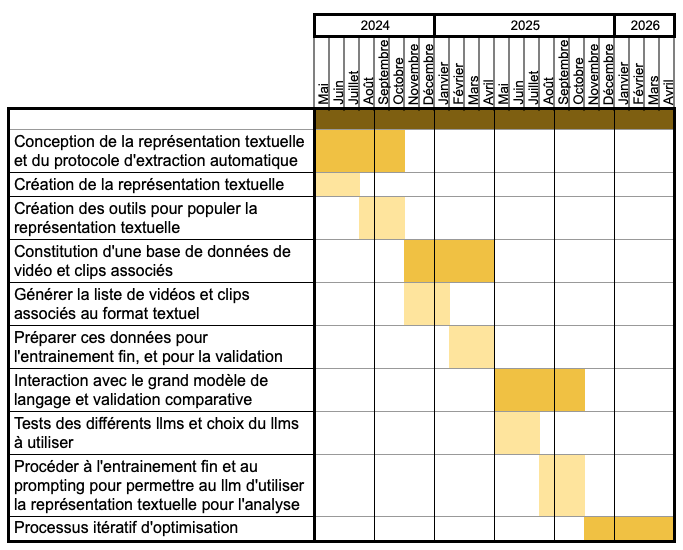
\includegraphics[width=\paperwidth]{gantt.png} % Replace 'image.jpg' with your image file name
    \caption{Échéancier du projet}
    \label{fig:label}
\end{figure}
\end{landscape}

\chapter{CONCLUSION}
Pour conclure, l'IAd représente une avancée prometteuse dans le domaine du montage vidéo automatisé, spécialement conçue pour répondre aux besoins des créateurs de contenu et des influenceurs en ligne. En s'appuyant sur des technologies de LLM et des techniques multimodales intégrant texte, image et audio, l'IAd permet de générer des clips optimisés pour l'engagement, tout en offrant des capacités de personnalisation pour répondre aux exigences spécifiques des utilisateurs.
En comparaison avec les solutions existantes, l'IAd se distingue par sa capacité à combiner une sélection automatique des moments pertinents avec des options de personnalisation avancées, une adaptabilité aux tendances en temps réel, et une flexibilité pour traiter divers types de contenu. Ces atouts rendent l'outil particulièrement précieux dans le contexte actuel du marketing d'influence, où la rapidité de production et la qualité des clips sont des facteurs clés de succès.
L'intégration de systèmes de rétroaction et de tests A/B assure également une amélioration continue de l'IA, lui permettant de s'adapter aux changements des préférences de l'audience et d'optimiser constamment ses décisions pour maximiser l'impact des vidéos. En résumé, l'IAd propose une solution innovante et adaptable, positionnée pour devenir un outil indispensable pour les créateurs de contenu souhaitant augmenter leur visibilité tout en réduisant les coûts de production


\end{document}